\documentclass[12pt]{article}
\usepackage[english]{babel}
\usepackage{float}
\usepackage[margin=1in]{geometry}
\usepackage{graphicx}
%\usepackage[toc,page]{appendix}
\graphicspath{ {./img/} }
\newcommand{\rpm}{\raisebox{.2ex}{$\scriptstyle\pm$}} 
\usepackage{listings}
\usepackage{xcolor}
\usepackage{indentfirst}
\usepackage{caption}
\usepackage[final]{pdfpages}
\usepackage{amsmath}
\usepackage[normalem]{ulem}



\begin{document}

\title{Joe Phaneuf \\ Computer Vision 16-720 Spring 2018 Homework 3 \\ Mar. 7, 2018 }
\date{}
\author{}
\maketitle

\newpage


%\stepcounter{section}
%%%%%%%%%%%%%%%%%%%%%%%%%%%%%%%%%%%%%%%%%%%%%%%%%%%%%%%%%%%%%%%%%%%%%%%%%%%%%%%%
%%%%%%%%%%%%%%%%%%%%%%%%%%%%%%%%%%%%%%%%%%%%%%%%%%%%%%%%%%%%%%%%%%%%%%%%%%%%%%%%
\section{Q1}
\subsection{Q1.1}
Let us not think about image planes for just a moment. Say P is some 3D point on a plane $\Pi$. We also assign a coordinate frame frame $\Pi$ , and we can use a 4x4 homogeneous transform matrix $H_{\Pi}^{p}$ to express point P in another frame that we will confusingly label p. We can also do this for yet another frame q with $H_{\Pi}^{q}$. These transform matrices encapsulate 3D rotations and translations, and are invertible. If we know P in frame q ( call it $P^{q}$ ) , we can express it in frame p as $P^{p} = H_{\Pi}^{p} H_{q}^{\Pi} P^{q}$. Because we know how to multiply matrices, we can collapse $H_{\Pi}^{p}$ and  $H_{q}^{\Pi}$ into one 4x4 matrix $H_{q}^{p}$.

Since we are arbitrarily assigning frames to things, we say that the Z axis of our $\Pi$ frame is normal to the $\Pi$ plane, and the plane is at Z=0. The consequence of this is that during coordinate transofmrations the Z value of a point on $\Pi$ is always 0, meaning the third column of $H_{q}^{p}$ does absolutely nothing and we can throw it away. Also, we would like to convert to homogeneous 2d coordinates, so the last row of $H_{q}^{p}$ can also be thrown away.

$$
H_{q}^{p}=
\begin{bmatrix}
h_{11} & h_{12} & h_{13} & h_{14} \\
h_{21} & h_{22} & h_{23} & h_{24} \\
h_{31} & h_{32} & h_{33} & h_{34} \\
0 & 0 & 0 & 1
\end{bmatrix}
\begin{bmatrix}
X \\ Y \\ Z \\ 1
\end{bmatrix}
\rightarrow
H_{2d}=
\begin{bmatrix}
h_{11} & h_{12} & h_{14} \\
h_{21} & h_{22} & h_{24} \\
h_{31} & h_{32} & h_{34} 
\end{bmatrix}
\begin{bmatrix}
X \\ Y  \\ 1
\end{bmatrix}
$$

So what does this mean? This means we can map a point on a fixed plane from a camera frame to a different camera frame with a 3x3 transform matrix, with the caveat that depth information is not preserved. The intrinsic camera matrices can then be used to map to and from the cameras' respective image planes in homogeneous coordinates, and X,Y values extracted.

\begin{figure}[H]
\centering
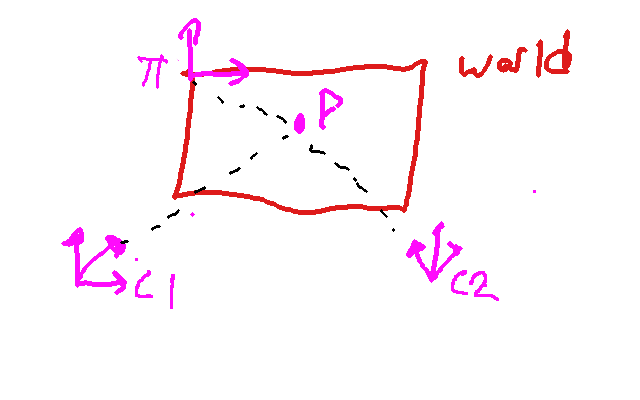
\includegraphics[page=1,width=0.75\textwidth]{q1_1a}
\caption{ Camera Frames observing point on plane } 
\label{fig:autoencout}
\end{figure}   


\subsection{Q1.2}
Consider two cameras that are separated purely by rotation. That is, the cameras' coordinate frames share an origin and a Z axis, and camera frame 2 is offset from camera frame 1 by a rotation about the Z axis. If we know intrinsic camera parameters ( $K_{1}$ and $K_{2}$ for cameras 1 and 2 ) , we can map points in the cameras' image planes to their respective camera frames. Because the camera frames are separated by a rotation only, the x and y values of a point in frame 1 are only a function of the x and y values of the point in frame 2. Breaking the notation of the homework handout, a point in camera frame 1 can be calculated as a linear function of a point in camera frame 2 like so:
$$
\textbf{x}_{1} = 
\begin{bmatrix}
x_{1} \\ y_{1} \\ 1
\end{bmatrix}
=
\begin{bmatrix}
f_{x} ( x_{2} , y_{2} ) \\
f_{y} ( x_{2} , y_{2} ) \\
1
\end{bmatrix}
$$
Which can be written generically as a 3x3 transform matrix:
$$
\textbf{x}_{1} = 
\begin{bmatrix}
h_{11} & h_{12} & h_{13} \\
h_{21} & h_{22} & h_{23} \\
0 & 0 & 1
\end{bmatrix}
\textbf{x}_{2}
$$
Note that in this particular situation, this should actually take the form of a 3x3 2 dimensional transform matrix parameterized by an angle $\theta$.
$$
\textbf{x}_{1} = 
\begin{bmatrix}
cos \theta & 0           & 0 \\
0          & sin \theta  & 0 \\
0          & 0           & 1
\end{bmatrix}
\textbf{x}_{2}
$$

\subsection{Q1.3}
\subsubsection{Q1.3.1}
Consider a transform matrix H that maps a point from one image plane to another image plane. Ignoring all other frames ( camera , world, or otherwise ) , 6 degrees of freedom are required to describe the rotation and translation from one frame to another (3 for translation, 3 for rotation). In the case of cameras, changes in focal length will create a scaling effect in the X and Y directions, which amounts to 2 degrees of freedom. All in, that H has 8 degrees of freedom.
\subsubsection{Q1.3.2}
Each image point contains two pieces of information. 4 points are therefore required to solve for the transformation matrix described in the preceeding subsection.
\subsubsection{Q1.3.3}
$$
\textbf{x}^{i}_{1}=
\begin{bmatrix}
x^{ \prime } \\ y ^ { \prime } \\ 1
\end{bmatrix}
$$

$$
\textbf{x}^{i}_{2}=
\begin{bmatrix}
x \\ y \\ 1
\end{bmatrix}
$$

$$
\textbf{x}^{i}_{1}=
\alpha
\textbf{H}
\textbf{x}^{i}_{2}
=
\alpha
\begin{bmatrix}
h_{11} & h_{12} & h_{13} \\
h_{21} & h_{22} & h_{23} \\
h_{31} & h_{32} & h_{33} 
\end{bmatrix}
\textbf{x}^{i}_{2}
$$

$$
\textbf{x}^{i}_{1}=
\begin{bmatrix}
x^{ \prime } \\ y ^ { \prime } \\ 1
\end{bmatrix}
=
\begin{bmatrix}
\alpha ( h_{11} x + h_{12} y + h_{13} ) \\
\alpha ( h_{21} x + h_{22} y + h_{23} ) \\
\alpha ( h_{31} x + h_{32} y + h_{33} )
\end{bmatrix}
$$

$$
\begin{bmatrix}
( h_{31} x + h_{32} y + h_{33} ) x^{ \prime } \\ 
( h_{31} x + h_{32} y + h_{33} ) y^ { \prime } 
\end{bmatrix}
=
\begin{bmatrix}
( h_{11} x + h_{12} y + h_{13} ) \\
( h_{21} x + h_{22} y + h_{23} )
\end{bmatrix}
$$

$$
\begin{bmatrix}
( h_{31} x + h_{32} y + h_{33} ) x^{ \prime } - ( h_{11} x + h_{12} y + h_{13} ) \\
( h_{31} x + h_{32} y + h_{33} ) y^{ \prime } - ( h_{21} x + h_{22} y + h_{23} )
\end{bmatrix}
=
\begin{bmatrix}
0 \\ 0
\end{bmatrix}
$$

$$
\begin{bmatrix}
- h_{11} x 
- h_{12} y 
- h_{13}
+ 0 + 0 + 0
+ h_{31} x  x^{ \prime }
+ h_{32} y  x^{ \prime }
+ h_{33} x^{ \prime }   \\
0 + 0 + 0
- h_{21} x 
- h_{22} y 
- h_{23}
+ h_{31} x y^{ \prime } 
+ h_{32} y y^{ \prime } 
+ h_{33}   y^{ \prime } 
\end{bmatrix}
=
\begin{bmatrix}
0 \\ 0
\end{bmatrix}
$$

$$
\textbf { h } = 
\begin{bmatrix}
h_{11} & h_{12} & h_{13} & h_{21} & h_{22} & h_{23} & h_{31} & h_{32} & h_{33} 
\end{bmatrix}^{T}
$$

$$
\textbf{A}_{i} = 
\begin{bmatrix}
- x 
- y 
- 1
+ 0 + 0 + 0
+ x  x^{ \prime }
+ y  x^{ \prime }
+ x^{ \prime }   \\
0 + 0 + 0
- x 
- y 
- 1
+ x y^{ \prime } 
+ y y^{ \prime } 
+   y^{ \prime } 
\end{bmatrix}
=
\begin{bmatrix}
0 \\ 0
\end{bmatrix}
$$

$$
\textbf{A}_{i} 
\textbf { h } =  \textbf { 0 }
$$
\end{document}


